%% Background
\chapter{Background}
\label{chap:background}

\section{Neural Machine Translation}

Neural networks can be adapted for many different tasks, and those tasks can be categorized by the type of input and the type of output. For example, spam detection iis a “sequence classification” task in which the input is a sequence (in this case, of words) and the output is a boolean value (in this case, whether the input is a spam email). Translation is a sequence-to-sequence task, because the input sequence (e.g. a sentence in French) is mapped to an output sequence (e.g. an English translation of that sentence). The input and output sequences can differ from one another in length, in script, and in syntactic structure.

How would it work to individually translate words in a source sentence and combine them according to the target language’s syntax rules? It would often provide a terrible translation, not just because different languages can communicate the same information in more or fewer words than one another; words cannot be translated individually because their meanings depend on their context. The same preposition, “in,” may correspond to any of several German prepositions – “in” or “auf” or “bei” – depending on the context. Thus effective translation of a single word in context may require use of an entire sentence or more than one sentence.

\section{The Transformer Model}

The Transformer model \cite{vaswani2017attention} innovated on the encoder-decoder structure \cite{sutskever2014sequence}, and has become the standard for NMT architecture. It uses an attention \cite{bahdanau2014neural} and positional encodings in place of recurrence. This new architecture trains much more quickly as it allows for more parallelizable training, and it is better at modeling long-range dependencies between sequence elements. Consider the following German sentence and its English translation:

\begin{itemize}
\item{Ich habe die alte graue mittelaltliche Burg gesehen. }

\item{I have seen the old gray medieval castle. }
\end{itemize}

The German version has the past participle "gesehen" (seen) at the very end of the sentence, separated from the modal verb "haben" (have). This is a long-range dependency; accurate translation requires comprehension of the entire sentence, not just a word or two at a time. 

In the following section, I'll describe at a high level how a Transformer model translates a sentence.

\vskip.25in
\underline{Tokenize}

The sentence must first be broken down into small parts for the model to work with. This is done with the tokenizer, which is often itself a trained component of the model. The tokenizer's vocabulary contains enough words and sub-words to cover the languages the model takes as input. Thus the tokenizer turns the sentence into a list of tokens, which are all elements in the tokenizer's vocabulary. Here is the result of tokenizing the sentence Consider the English sentence "The man wearing black shoes rode his bicycle." using the tokenizer for Meta's NLLB models:
\vskip.25in

   [256047, 1617, 492, 214030, 49154, 203020, 134457, 4414, 330, 163731, 248075, 2]
  
   ['eng\_Latn', 'The', 'man', 'wearing', 'black', 'shoes', 'rode', 'his', 'bi', 'cycle', '.', '</s>']

\vskip.25in
The integer array contains the indices of the tokens in the tokenizer's vocabulary. Note the inclusion of two special token:
\begin{itemize}
    \item{'</s>,' is an "end of sentence" token which the tokenizer adds to every input. } 
    \item{‘eng\_Latn’ is the language tag, also added during tokenization. The language tag does not affect how the tokenizer breaks up the sentence, rather, it presence is meant for the encoder.}
    
\end{itemize}

\vskip.25in
\underline{Encode}

In its first layer, the encoder deterministically turns each token into a dense vector embedding, then implicitly marks the position of each token in the sentence by adding a unique sum of sinusoids. The embedding vectors corresponding to each token in the vocabulary are learned in training, and the model learns the implicit meaning of the signal added by the positional encoding. The rest of the layers of the encoder repeatedly use self-attention to contextualize each embedding in the sentence. The embedding of a verb might be strongly influenced by the noun it is acting on, or the embedding of an article in a gendered language might depend primarily on the gender of its referent, for example.

\vskip.25in
\underline{Decode}

The decoder uses the vector embeddings to generate probabilities for tokens in the tokenizer’s vocabulary. There are different strategies for token selection - using the token with the highest probability every time (greedy selection) is the most common. The decoder uses attention to the tokens it has already generated to generate each new token. 

\section{Exploratory Experiments}

The beginning portion of this project was spent trying to understand and use the NLLB models. The full sized model has 54.5 billion parameters, which is far too large for the available hardware, but Meta also published smaller versions of the model with 3.3 billion, 1.3 billion, and 600 million parameters. An early goal was to fine-tune one of these smaller models with a language not represented in the original 200. Fine-tuning is the process of training a pre-trained model to improve its performance on a particular task or set of tasks. The language pair chosen for these early experiments is unimportant, as the goal was to determine the general procedure of finetuning and become familiar with the necessary Python libraries. After some time experimenting on the language pair Russian-Tyvan (a turkic language with strong Russian influence), I arrived at basic code for NLLB model fine-tuning. After some number of updates (I used 1,000), the model was saved if it showed better performance than at the last checkpoint. This was repeated over 60,000 updates, but to save time, the training terminated if no progress had been made in 30,000 updates.

The training loop relies on the model's loss to evaluate performance, but this score does not represent the accuracy of the translations. Evaluating translations is a difficult task in its own right… most sentences could be accurately translated in several ways. Any algorithm for this task will be imperfect, but the use of the Bilingual Evaluation Understudy (Bleu) and the Character n-gram F-score (chrF++) are standard in the field of NMT. To evaluate the model’s performance after fine-tuning, sentences from the dev set are translated (in both/all directions) and the translations are compared to those provided in the dataset using Bleu and chrF++. 

I fine-tuned a number of other models using training data from the AmericasNLP dataset (cite?), which contains indigenous languages from North, Central, and South America, each paired with Spanish. The results were, in general, lower than but comparable to the scores submitted by researchers at the University of Sheffield \cite{gow2023sheffield}. The lower scores were acceptable given that the task at hand was not to submit scores to the annual AmericasNLP conference. I also developed code for multilingual training and evaluation with this set of languages, which involves the use of all language pairs and directions. 

\section{Digging into the Embedding Space}

With a solid foundation in fine-tuning and model evaluation, I turned my focus to the embedding space of the NLLB models in an attempt to generate insights into the relationship between the vector representations of tokens and sentences before decoding. To capture these vectors for experimentation, I cloned the NLLB architectures with a layer inserted to take a “snapshot” of the vector embeddings after encoding. These were the contextual embeddings of the original tokens - whereas "bat" would be tokenized identically in the phrases "baseball bat" and "vampire bat," the contextual embeddings would be completely different.

The vectors produced by the encoder are high dimensional and therefore impossible to imagine or plot in 2- or 3-dimensional space. But understanding the relationship between embeddings within and across languages seems an obvious prerequisite to the exploitation of transfer learning in multilingual settings. Interesting observations can be made without complex math or statistics, for example, that the cosine similarity (angle) between vectors can represent specific relationships between pairs of words. If we individually encode all the words in the English dictionary, then calculate the angle between the embedings of "man" and "king," we can guess at an analogy by adding that angle to the embedding of another word, say, "woman" and finding the nearest word to this new position. Indeed, we get "queen." In other words, the angle between the embeddings of "man" and "king" is close to the angle between the embeddings of "woman" and "queen." What does this emergent behavious indicate about the spatial organization of semantic meaning in the model, and what what other patterns are hidden in the embeddings?

Armed with the "seed" dataset of just over 6,000 sentences translated into 38 languages as well as the modified NLLB model, I began to investigate the relationships between vector embeddings. Since each sentence contains several tokens, I used an average of all of a sentence's tokens' embeddings to represent each sentence. I wanted to visualize these averaged sentence embeddings in 2D space to see whether any clustering patterns were obvious. Visualization required a reduction in dimensions, however, because the embedding vectors were of dimension 1,024. I used t-distributed stochastic neighbor embedding (t-SNE) \cite{van2008visualizing}, which provides a such reduction while preserving the structure of the points in space. To avoid overcrowding the graphs, I found that it was necessary to limit the number of points -- this meant either displaying only ten or twenty sentences in all 38 languages or displaying hundreds of sentences in only a few languages. See figure 2.1 for the results of these reductions and colored the points both by their sentence ID and by their language. 

\begin{figure}[ht]
    \centering
    \begin{subfigure}[b]{0.9\textwidth}

        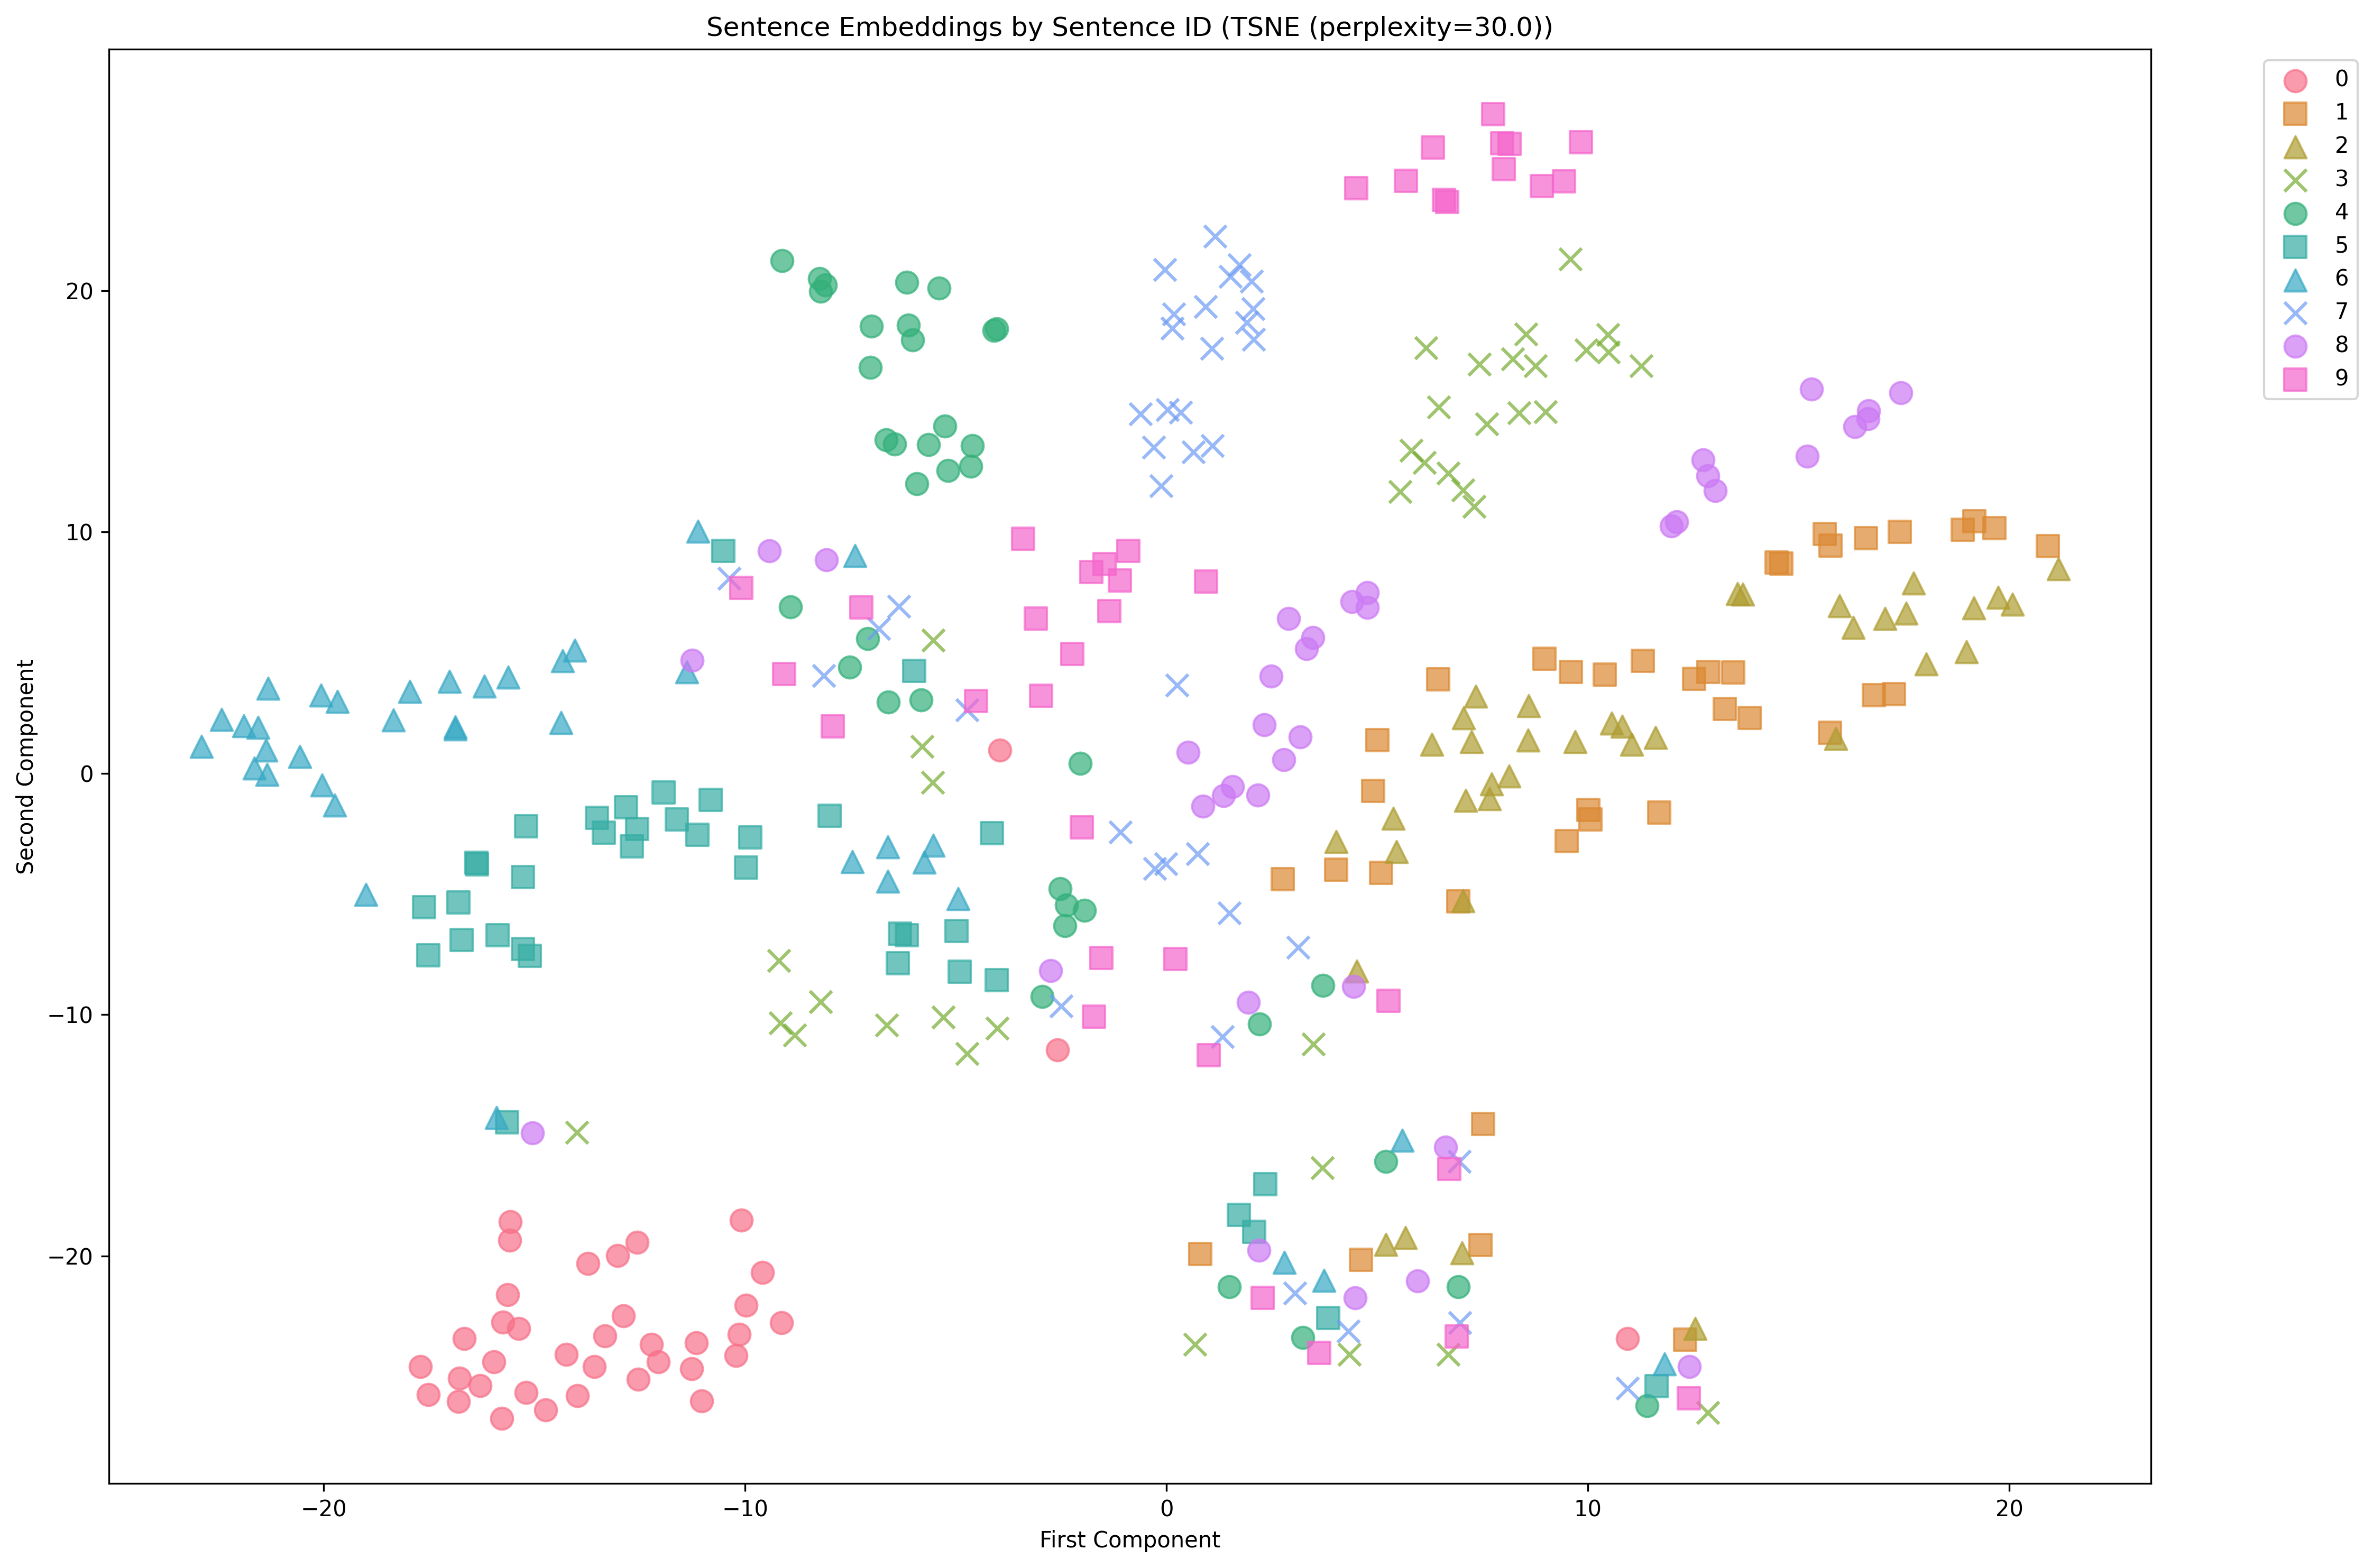
\includegraphics[width=\textwidth]{chapters/images/by_id.png}
        \caption{Colored by sentence ID}
        \label{fig:10sentsalllangsbyid}
    \end{subfigure}
    \hfill
    \begin{subfigure}[b]{0.9\textwidth}

        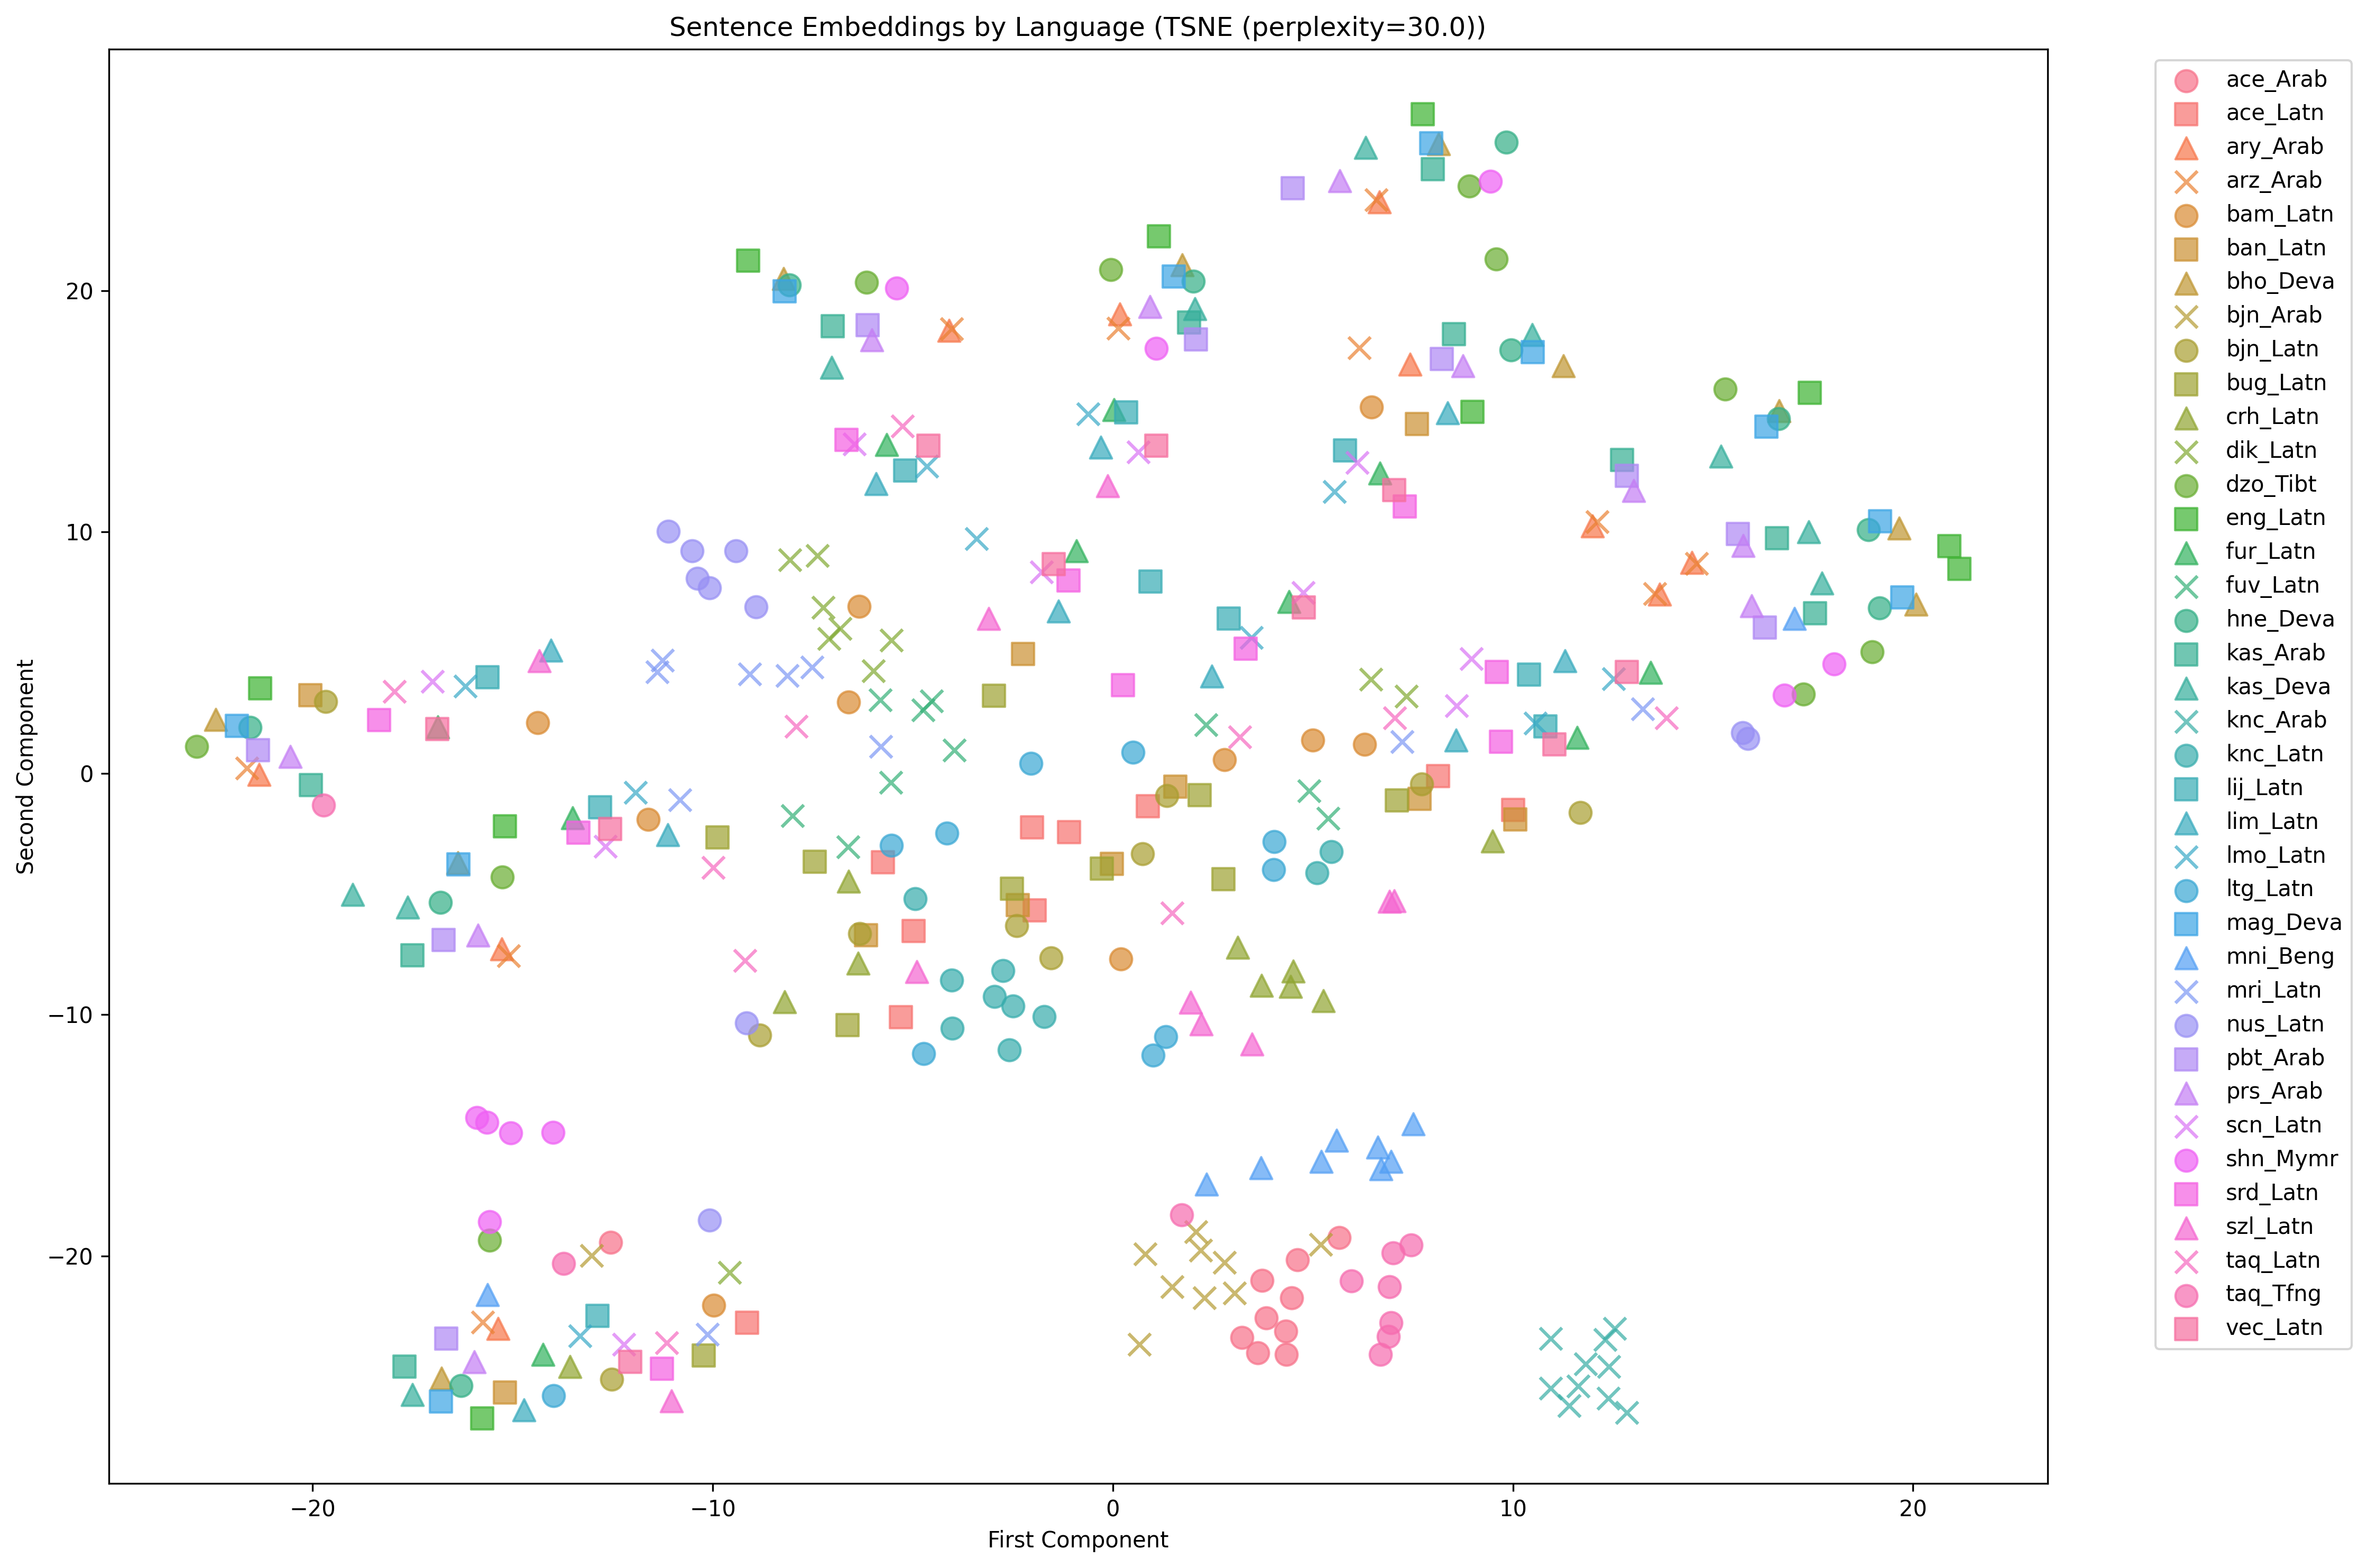
\includegraphics[width=\textwidth]{chapters/images/by_lang.png}
        \caption{Colored by language}
        \label{fig:10sentsalllangsbylang}
    \end{subfigure}
    
    \caption{t-SNE reduction of averaged sentence embeddings for 10 sentences and 38 languages}
    \label{fig:bothimages}
\end{figure}


The coloring by sentence ID shows much stronger clustering patterns, which makes sense. The embedding of each input will be treated the same by the decoder, regardless of the source language, so very similar embedding vectors will lead to very similar or identical translations. It is clear in the plots that the clustering is not perfect. Look at the cluster in the lower right corner of the ID-colored graph. This jumble represents several different sentences whose averaged encodings are very similar despite their distinct meanings. Looking to the language-colored graph sheds some light on the phenomenon: these are all knc\_Latn sentences (Central Kanuri in Latin script). All ten knc\_Latn sentences have very similar representations, and we should expect the decodings of these sentences to be similar to one another and different from translations of the same sentence from different source languages. Indeed, knc\_Latn performs very poorly in general, achieving a Bleu score of 1.757 and chrF++ score of 17.812 when translated with the 600 million parameter NLLB model. The averages over all the seed languages are 10.019 and 36.696 for Bleu and chrF++ respectively. 

